\documentclass[12pt,svgnames,table]{beamer}
\usetheme{progressbar}

\usepackage[utf8x,utf8]{inputenc}
\usepackage{tikz}
\usetikzlibrary{decorations.pathmorphing}
\usepackage{xcolor}
\usepackage{amsmath,amsfonts,amsthm, amssymb}
\usepackage[babel=true]{csquotes}
\usepackage{etoolbox}
\usepackage{dsfont}
\usepackage{chngpage}


\usepackage{graphics} %% TOUT NEW!!
\usepackage{pgfplots} %% TOUT NEW!!  virer si pbm

\usetikzlibrary{shapes,snakes}

%\usepackage{txfonts}
%\usepackage{MnSymbol} % symbol independent
\newcommand{\paren}[1]{\left( \left. #1 \right. \right)} 
\newcommand{\croch}[1]{\left[ \left. #1 \right. \right]} 
\newcommand{\set}[1]{\left\{ \left. #1 \right. \right\}}
\newcommand{\sachant}{\, \right| \left. \,}
\newcommand{\nico}[1]{ }
\newcommand{\nicoo}[1]{#1}
% Modifiez ou necessaire:
% titre de these/topo

\title{
\vspace{0.7cm}\\
Mixed-initiative mission planning\\ 
considering human operator state estimation\\ 
based on physiological sensors}

\normalsize
\author{\vspace{2cm} \textbf{Nicolas Drougard}}
% X=annee de these, Y=departement
\def\aboutauthor{\vspace{0.2cm}\hspace{-2.55cm} 
%under \textbf{D.Dubois}, \textbf{J-L.Farges} and \textbf{F.Teichteil-K\"onigsbuch} supervision\\
%\vspace{0.1cm}\hspace{-2.4cm} \textbf{doctoral school:} EDSYS \hspace{0.2cm} \textbf{institution:} ISAE--SUPAERO\\
%\vspace{0.1cm}\hspace{-3.2cm}\textbf{laboratory:} ONERA--The French Aerospace Lab\\ 
%\vspace{0.5cm} \hspace{0.2cm} 
\includegraphics[scale=0.45]{logo2015} \hspace{4.8cm}
%\begin{tikzpicture}
%\node[opacity=1] at (0,0) {\includegraphics[scale=0.35]{Logo_EDSYS2}};
%\end{tikzpicture}
}

% directeur de these
%\def\directeur{Toulouse}
% encadrant; s'il n'y a pas d'encadrant, veuillez commenter la ligne ci-dessous
%\def\encadrant{DCSD}


% Debut du documment
\begin{document}

% la premiere page
{
\usebackgroundtemplate{
\includegraphics[width=\paperwidth,height=\paperheight]{image_fond}} 
\begin{frame}[plain]
	\titlepage
\end{frame}
}



\section[context]{Context and Goal}

\begin{frame}
\frametitle{\insertsection} 
\framesubtitle{\footnotesize Human-machine systems}
\begin{block}{Increasing use of automated systems}
aircrafts, cars, unmanned vehicles (military operation, contaminated area), ... \\
\end{block}
\visible<2->{
\begin{itemize}
\item \textbf{Increasingly autonomous robots:}\\ 
technical advances in AI, machine learning, vision, decision ...
%deterministic behavior conditional to feedbacks/observations (policies)
\visible<3->{
\item \textbf{Human operator still vital:}\\
%more powerful for a vast majority of tasks 
- produces tactical and ethical decisions \\
- handles complex/unknown situations/systems
%(robot can apply optimal decisions for known systems)
}
\end{itemize}
}
\visible<4->{
\begin{alertblock}{}
Human factors involved in $80\%$ of AAVs accidents! \cite{Williams04asummary}
\end{alertblock}
}
\end{frame}

\begin{frame}
\frametitle{\insertsection} 
\framesubtitle{\footnotesize Human operator weaknesses}
\textbf{Potential effects of a mission on human operators:}
\begin{itemize}
\item stress (danger, pressure)
\item workload (multi-task, hard tasks)
\item fatigue, boredom (long mission)
\end{itemize}
\visible<2->{
\textbf{Consequences:}
\begin{itemize}
\item mental confusion
\item attentional tunneling
\item mind wandering
\item lower vigilance
\item ...
\end{itemize}
}
\visible<2->{
\begin{alertblock}{}
\center increase in accident risk resulting in mission fails 
\end{alertblock}
}
\end{frame}
\begin{frame}
\frametitle{\insertsection}
\framesubtitle{\footnotesize use of human state feedbacks!}
\begin{block}{Human operators equipped with sensors}
\center data from the human operator state can\\  
\textbf{refine supervision of human-robot team}
\end{block}
\visible<2->{
\begin{itemize}
\item \cite{Souza:2015:MTS:2921564.2921916} target identification task (ground robot)\\ 
- \textbf{devices:} eye tracking + electrocardiography\\% (ECG)\\
- \textbf{human state:} \textit{cognitive availability} {\color{DodgerBlue!70} estimation}\\ 
- \textbf{superv. validation:} {\color{DodgerBlue!70} simulations} of the system\\
\hspace{3.8cm} (including human behavior)
\end{itemize}
}
\visible<3->{
\begin{itemize}
\item \cite{DBLP:2016:conf/iros/GateauCLD16} search and rescue task (AAVs)\\ 
- \textbf{device:} eye tracking\\
- \textbf{human state:} \textit{current human task} {\color{DodgerBlue!70} = } human gaze \\% (deterministic)\\
- \textbf{superv. validation:} tested on 10 {\color{DodgerBlue!70} volunteers } 
\end{itemize}
}
\end{frame}


\begin{frame}
\frametitle{\insertsection}
\framesubtitle{\footnotesize work on progress}
\begin{alertblock}{Next stage}
\begin{itemize}
\item \textbf{devices:} eye tracking + electrocardiography ( + EEG, NIRS, ...)\\
\item \textbf{human state:} {\color{DodgerBlue!70} estimation } of - cognitive availability \\
\hspace{5cm} - current human task \\
\hspace{5cm} - type of human behavior \\
\hspace{8cm} \cite{Nikolaidis:2015:EML:2696454.2696455}\\
\visible<2->{
or any human relevant feature (situation awareness, involvement in the mission, ...)
}
\visible<3->{
\item \textbf{superv. validation:} test on {\color{DodgerBlue!70} volunteers} at ISAE\\ 
\hspace{3cm} on a mission rated with a \textbf{simple score}
}
\end{itemize}
\end{alertblock}
\visible<4->{
\begin{block}{}
robot/supervision sequential decisions computation: POMDP
\end{block}
}
\end{frame}



\section[uncertainty theories]{Alternative uncertainty theories}



\begin{frame}
\frametitle{\insertsection} 
\framesubtitle{\footnotesize Imprecision modeling}
imprecise expert information on unavailable $\textbf{p}$?\\
small number of volunteers?
\begin{itemize}
\item poor statistical analysis
\item low level confidence on computed $\textbf{p}$
\end{itemize}
\visible<2->{
$\rightarrow$ model imprecision using alternative uncertainty theories \cite{DBLP:conf/sum/DrougardDFT15}
\nico{ statistiques avec peu de participants!! $\rightarrow$ other uncertainty theories }
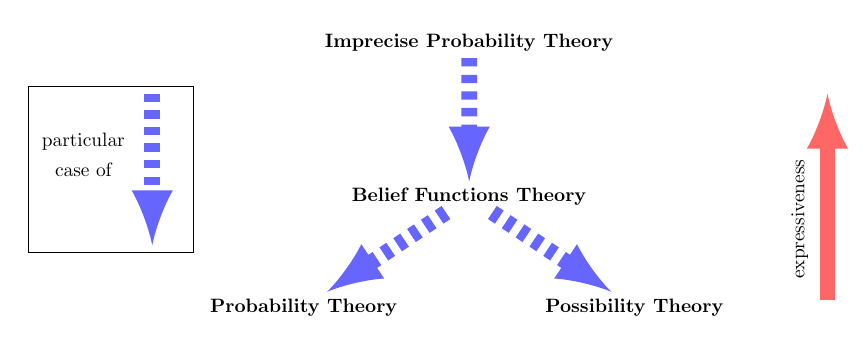
\begin{tikzpicture}[scale=0.7,transform shape]
\node (IP) at (2,10.8) {\textbf{Imprecise Probability Theory} };
\node (BF) at (2,8) {\textbf{Belief Functions Theory}};
\node (PROB) at (-1,6) {\textbf{Probability Theory}};
\node (POSS) at (5,6) {\textbf{Possibility Theory}};
\draw[->,>=latex,thick, color=blue!60, line width=2mm, dashed] (IP) to (BF);
\draw[->,>=latex,thick, color=blue!60, line width=2mm, dashed] (BF) to (PROB);
\draw[->,>=latex,thick, color=blue!60, line width=2mm, dashed] (BF) to (POSS);

\node (topr) at (8.5,10) {};
\node (botr) at (8.5,6) {};
\node (middr) at (8,7.6) [rotate=90] {expressiveness};
\draw[->,>=latex,thick, color=red!60, line width=2mm] (botr) to (topr);
\draw (-6,7) rectangle (-3,10);
\node (toplegend) at (-3.75,10) {};
\node (botlegend) at (-3.75,7) {};
\draw[->,>=latex,thick, color=blue!60, line width=2mm, dashed] (toplegend) to (botlegend);
\node (bluelegend) at (-5,9) {particular};
\node (bluelegend) at (-5,8.5) {case of};
\end{tikzpicture}
}
\end{frame}



\begin{frame}
\frametitle{\insertsection} 
\framesubtitle{\footnotesize Qualitative Possibility Theory -- ($\max$,$\min$) ``tropical'' algebra}
\vspace{0.15cm}
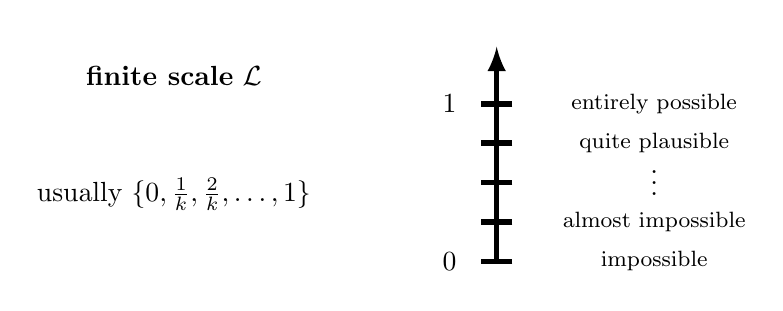
\begin{tikzpicture}
\node (top) at (1,2.5) {};
\node (bot) at (1,-0.5) {};
\draw[->,>=latex,line width=2pt] (bot) -- (top);
\node (finiteScale) at (-3.1,2) {\textbf{finite scale} $\mathcal{L}$};
\node (finiteScale2) at (-3.1,0.5) {usually $\{ 0, \frac{1}{k}, \frac{2}{k}, \ldots, 1 \}$};
\node at (0.4,1.65) {$1$};
\node at (3,1.65) {\footnotesize entirely possible};
\node at (3,1.15) {\footnotesize quite plausible};
\node at (3,0.75) {\vdots};
\node at (3,0.15) {\footnotesize almost impossible};
\node at (3,-0.35) {\footnotesize impossible};
\node at (0.4,-0.35) {$0$};
\draw[line width=2pt] (1.2,-0.35) -- (0.8,-0.35);
\draw[line width=2pt] (1.2,0.15) -- (0.8,0.15);
\draw[line width=2pt] (1.2,0.65) -- (0.8,0.65);
\draw[line width=2pt] (1.2,1.15) -- (0.8,1.15);
\draw[line width=2pt] (1.2,1.65) -- (0.8,1.65);
\end{tikzpicture}
%$1 = l_1 > l_2 > \ldots > l_{\# \mathcal{L}} = 0$ form the 
\begin{exampleblock}{}	
\flushleft events $E \subset \Omega$ (universe) \\ 
\centering
\textbf{sorted} using possibility \textbf{degrees} $\Pi(E) \in \mathcal{L}$ \\
	$\neq$ \\
	\textbf{quantified} with \textbf{frequencies} $\mathbb{P}(E) \in \croch{0,1}$ (probabilities)
	\end{exampleblock}
\visible<2->{
	\begin{block}{}
\vspace{-0.2cm}
\begin{center}
\[ \Pi(E) = \max_{e \in E} \Pi(\set{e}) = \max_{e \in E} \pi(e) \]
%	$e_1 \neq e_2$, $2$ events $\subset \Omega$ 
%	\begin{itemize}
%	\item $ \pi(e_1) < \pi(e_2) $ $\Leftrightarrow$ \textit{``$e_1$ 
%is less plausible than $e_2$''} \\
%	\end{itemize}	
\end{center}	
\end{block}
}
\end{frame}



\begin{frame}
\frametitle{\insertsection} 
\framesubtitle{\footnotesize joint work with \textbf{Sergio Pizziol} -- Context}
\vspace{0.1cm}
\begin{figure}
\centering
\begin{tikzpicture}[scale=1,transform shape]
%states
\tikzstyle{vertex}=[fill=black!20,draw=black,  minimum width=85pt,line width=1pt,inner sep=5pt, minimum height=60pt]
\tikzstyle{vertexBIG}=[fill=black!20,draw=black, minimum width=280pt, minimum height=40pt,line width=1pt,inner sep=5pt]

%% HMI
\node[vertex] (M) at (-1.5,-0.25) {};
\node () at (-1.1,0.5) {\textbf{Machine}};
\node[vertex] (H) at (5.5,-0.25) {};
\node () at (4.95,0.5) {\textbf{Human}};
\node () at (5.8,-0.47) {
\includegraphics[scale=0.05]{airplane-1295845_960_720}};
\node () at (-1,-0.6) {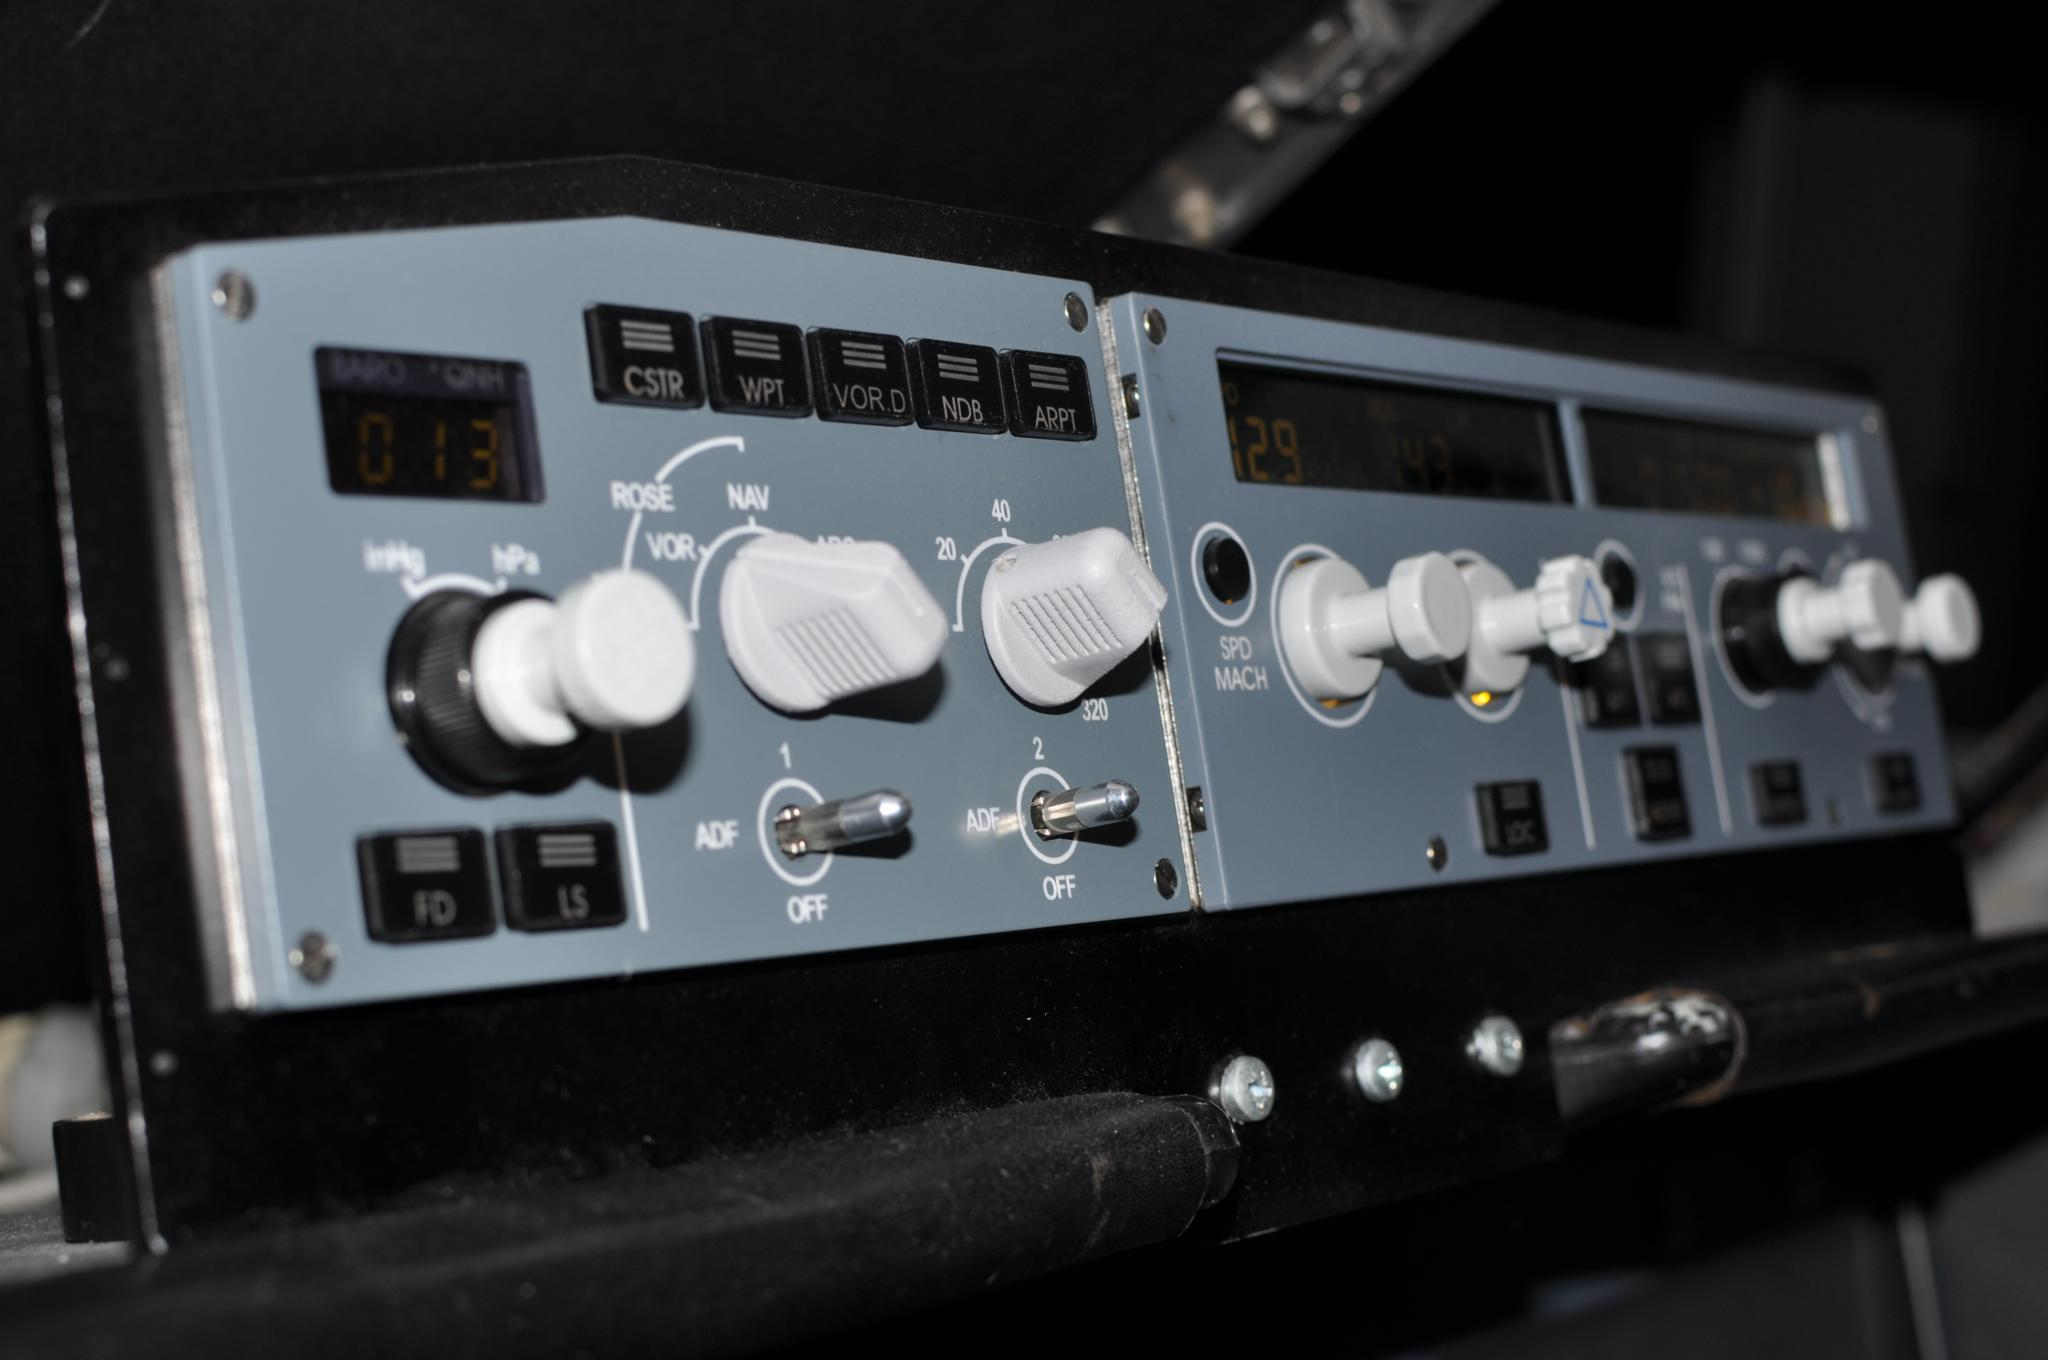
\includegraphics[scale=0.025]{fcu}};
\node () at (-2.45,-0.4) {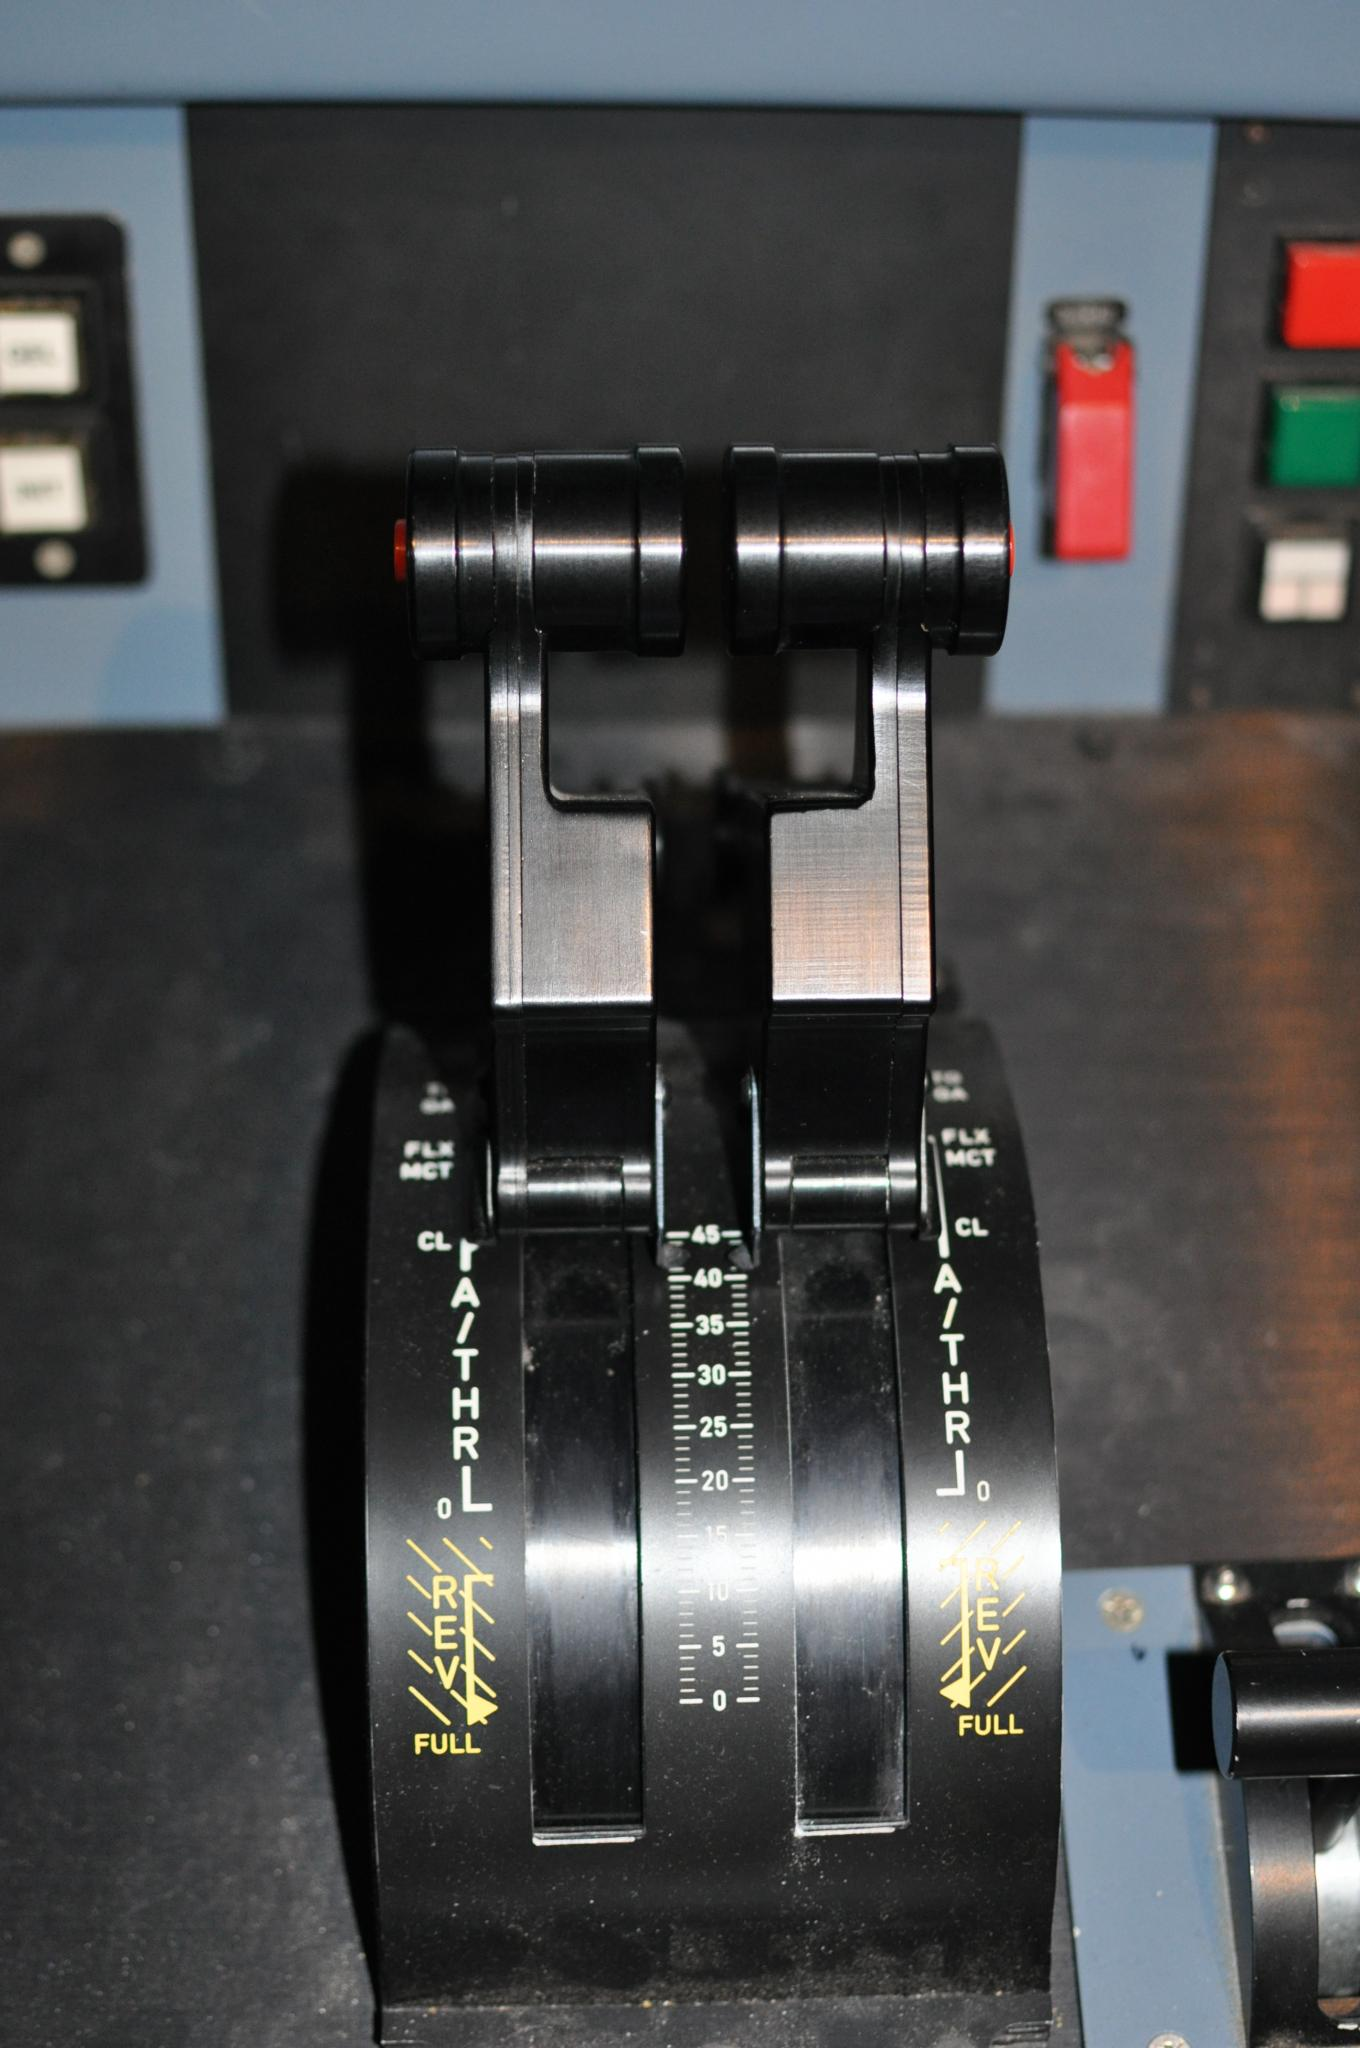
\includegraphics[scale=0.02]{manettegaz}};
%% ARROWS
\draw[->,>=latex,line width=4pt,color=red] (-0.15,0.3) -- (4.2,0.3);
\draw[->,>=latex,line width=4pt,color=red] (4.2,-1) -- (-0.15,-1);
%%LEGEND
\node () at (1,0.6) {\footnotesize Feedbacks};
\node () at (3,-0.4) {\footnotesize Interface};
\node () at (2.8,-0.75) {\footnotesize manipulations};

\visible<3->{
%% OBSERVER
\node[vertexBIG] (O) at (2,-2.5) {};
\node () at (1.9,-2.1) {\textbf{Observer}};
\definecolor{bbbbbblue}{rgb}{0,0.325,0.678}
\node[ellipse,draw, thick,fill=bbbbbblue!30] (el) at (-0.55,-2.7) {Machine model};
\node[ellipse,draw, thick,fill=bbbbbblue!30] (el) at (4.15,-2.7) {Human error model};

\draw[->,>=latex,line width=2pt,color=red, dashed] (3,-1) -- (3,-2);
\draw[->,>=latex,line width=2pt,color=red, dashed] (0.8,0.3) -- (0.8,-2);
}

\end{tikzpicture}
%\caption{ 3 actors involved: red arrows = information flows.}
\end{figure}
\vspace{-0.3cm}
\visible<2->{
\begin{block}{}
\textbf{Issue:} incorrect human assessment of the machine state \\ 
\hspace{2cm} $\rightarrow$ \textbf{accident risk}
\end{block}
}
\vspace{-0.15cm}
\visible<4->{
\begin{alertblock}{$\pi$-POMDP without actions: $\pi$-Hidden Markov Process}
\begin{itemize}
\item \textbf{system space} $\mathcal{S}$: set of human assessments $\rightarrow$ \textbf{hidden} 
\item \textbf{observation space} $\mathcal{O}$: feedbacks/human manipulations
\end{itemize}
\end{alertblock}
}
\end{frame}





\begin{frame}
\frametitle{\insertsection} 
\framesubtitle{\footnotesize Human error model from expert knowledge}
\vspace{0.2cm}
\begin{alertblock}{Machine with states $A$, $B$, $C$, $\ldots$}
state $s_A \in \mathcal{S}$: ``human thinks machine state is $A$'' 
\end{alertblock}
\visible<2->{
	\begin{exampleblock}{ Machine state transition $A \rightarrow B$}
	\begin{itemize}
		\item observation: \textbf{machine feedback} $o_f' \in \mathcal{O}$: 
	\end{itemize}
	\textit{``human usually aware of feedbacks''} $\rightarrow$ $\pi \paren{s_B',o_f' \sachant s_A} = 1$\\
	\hspace{1.5cm} \textit{``but may lose a feedback''} $\rightarrow$ $\pi \paren{s_A',o_f' \sachant s_A} = \frac{2}{3}$ 
	\visible<3->{
		\begin{itemize}
			\item  observation: \textbf{human manipulation} $o_m' \in \mathcal{O}$:
		\end{itemize}
		\textit{``manipulation $o_m'$ is normal under $s_A$''} $\rightarrow$ $\pi \paren{s_B',o_m' \sachant s_A} = 1$\\
		\hspace{2.8cm} \textit{``is abnormal''} \hspace{1.1cm} $\rightarrow $ \hspace{2cm} $ = \frac{1}{3}$ 
	}
	\visible<4->{
		\begin{itemize}
			\item impossible cases: possibility degree $0$
		\end{itemize}
	}
	\end{exampleblock}
}
\end{frame}



\begin{frame}
\frametitle{\insertsection} 
\framesubtitle{\footnotesize $\pi$-HMP, detection $\&$ diagnosis tool for HMI (with \textbf{Sergio Pizziol})}
\vspace{0.3cm}
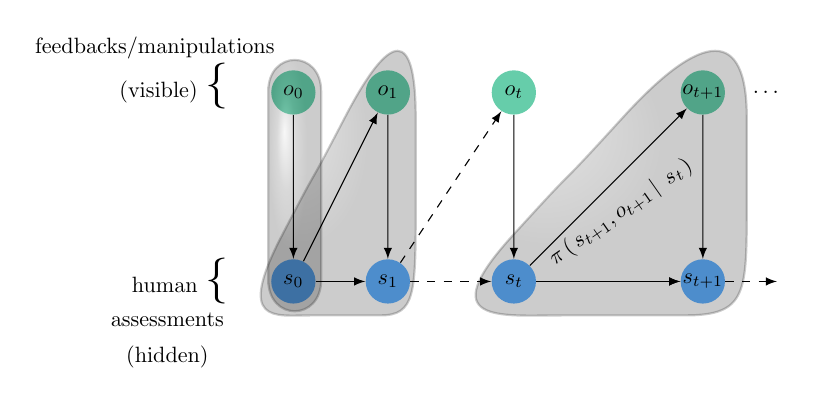
\begin{tikzpicture}[scale=0.8,transform shape]

%TIME
%\node [font=\huge] (statet) at (3.8,1) {$t$};
%\node [font=\huge] (statetplus1) at (8.9,1) {$t+1$};
%%%%%%%%%%%%%%%%%%%%%%%%%%%%%%%%%%%%%%%%%%%%%%%%%%%%%%%%%%%%%%%%%%%%%%%%
%states
\tikzstyle{vertex}=[circle,fill=DodgerBlue!70,minimum size=20pt,inner sep=0pt]
\tikzstyle{mvertex}=[circle,fill=DodgerBlue!70,minimum size=30pt,inner sep=0pt]
\tikzstyle{overtex}=[circle,fill=MediumAquamarine,minimum size=20pt,inner sep=0pt]


\node (Oc) at (0.8,3.7) {feedbacks/manipulations};
\node (V) at (1.1,3.1) {(visible) \huge $\{$};
%\node (V) at (1.5,1) {effects \huge $\{$};
\node (H) at (1.2,0) {human \huge $\{$};
\node (H1) at (1,-0.6) {assessments};
\node (H1) at (1,-1.2) {(hidden)};

%\node (E) at (1.7,1.5) {effects \huge $\{$};

%1
\node[overtex] (state1) at (3,3) {$o_0$};
%\node[vertex] (state11) at (2.5,1) {$e_0$};
\node[vertex] (state111) at (3,0) {$s_0$};
%2
\node[overtex] (state2) at (4.5,3) {$o_1$};
%\node[vertex] (state22) at (4,1) {$e_1$};
\node[vertex] (state222) at (4.5,0) {$s_1$};

\node[overtex] (state3) at (6.5,3) {$o_t$};
%\node[vertex] (state33) at (6,1) {$e_t$};
\node[vertex] (state333) at (6.5,0) {$s_t$};

\node (H) at (8.2,1.1) [rotate=35] {$\pi \paren{s_{t+1},o_{t+1} \sachant s_t}$};

\node[overtex] (state4) at (9.5,3) {$o_{t+1}$};
%\node[vertex] (state44) at (8,1) {$e_{t+1}$};
\node[vertex] (state444) at (9.5,0) {$s_{t+1}$};


\node (state23) at (10.5,3) {$\hdots$};

%3
\node (state5) at (10.8,2) {};
\node (state55) at (10.8,1) {};
\node (state555) at (10.8,0) {};

%\node (e0) at (2.9,1.6) [color=black!70] {\huge $e_0$};
%\node (e1) at (4.2,1.6) [color=black!70] {\huge $e_1$};
%\node (et) at (8.9,1.6) [color=black!70] {\huge $e_{t+1}$};

%SV
% arrows sv->sv
%1->2
\draw[->,>=latex] (state1) -- (state111);
\draw[->,>=latex] (state111) -- (state2);
\draw[->,>=latex] (state111) -- (state222);
%\draw[->,>=latex] (state111) -- (state11);
%\draw[->,>=latex] (state1) -- (state11);


\draw[->,>=latex] (state2) -- (state222);
\draw[->,>=latex,dashed] (state222) -- (state3);
\draw[->,>=latex,dashed] (state222) -- (state333);
%\draw[->,>=latex] (state2) -- (state22);
%\draw[->,>=latex] (state222) -- (state22);
%\draw[->,>=latex] (state111) -- (state22);

\draw[->,>=latex] (state3) -- (state333);
\draw[->,>=latex] (state333) -- (state444);
\draw[->,>=latex] (state333) -- (state4);

%\draw[->,>=latex] (state333) -- (state33);
%\draw[->,>=latex] (state3) -- (state33);
%\draw[->,>=latex,dashed] (state222) -- (state33);
\draw[->,>=latex] (state333) -- (state444);
\draw[->,>=latex] (state4) -- (state444);
\draw[->,>=latex,dashed] (state444) -- (state555);

%\draw[->,>=latex] (state444) -- (state44);
%\draw[->,>=latex] (state4) -- (state44);
%\draw[->,>=latex] (state333) -- (state44);

\draw [scale=0.7,xscale=1.4,ball color=black,opacity=0.2,xshift=40,yshift=35,thick=5pt]
 (9,2.5)..controls +(0,2) and +(1.3,2) ..(7,2.5) % angle haut
 ..controls +(-1.3,-2) and +(1.3,2) ..(5.2,-0.2) % ligne gauche inclinee
 ..controls +(-1.3,-2) and +(-1,0).. (6,-2) % angle inferieur gauche
 ..controls +(-1,0) and +(1,0).. (8,-2)
 ..controls +(1,0) and +(0,-2).. (9,0.5) % angle inferieur droit
 ..controls +(0,1) and +(0,-1).. (9,2.5); % arc 4

\draw [scale=0.7,xscale=0.8,ball color=black,opacity=0.2,xshift=-5,yshift=35,thick=5pt]
 (9,2.5)..controls +(0,2) and +(1.3,2) ..(7,2.5) % angle haut
 ..controls +(-1.3,-2) and +(1.3,2) ..(5.2,-0.2) % ligne gauche inclinee
 ..controls +(-1.3,-2) and +(-1,0).. (6,-2) % angle inferieur gauche
 ..controls +(-1,0) and +(1,0).. (8,-2)
 ..controls +(1,0) and +(0,-2).. (9,0.5) % angle inferieur droit
 ..controls +(0,1) and +(0,-1).. (9,2.5); % arc 4


\draw [scale=0.7,xscale=0.8,yscale=0.95,ball color=black,opacity=0.2,xshift=-67,yshift=58,thick=5pt]
 (8.5,2.5)..controls +(0,1) and +(0,1) ..(7,2.5) % angle haut
 ..controls +(0,1) and +(0,-1) ..(7,-2) 
 ..controls +(0,-1) and +(0,-1).. (8.5,-2) % angle inferieur droit
 ..controls +(0,1) and +(0,-1).. (8.5,2.5); % arc 4

%%%%%%%%%%%%%%%%%%%%%%%%%%%%%%%%%%%%%%%%%%%%%%%%%%%%%%%%%%%%%%
% TRANSITION FUNCTIONS
%\node (T1) at (7.1,2.05) {$T^{a,1}$};
%\node (T2) at (7,1.45) {$T^{a,2}$};
\end{tikzpicture}
\visible<2->{
\begin{itemize}
\item \textbf{estimation} of the human assessment\\
\hspace{3cm}$\Leftrightarrow$ \textbf{possibilistic belief state}% over $s \in \mathcal{S}$ 
\item \textbf{detection} of human assessment errors + \textbf{diagnosis}
\item validated with pilots on flight simulator missions
\end{itemize}
}
\end{frame}


\begin{frame}
        \frametitle{\hspace{0.3cm} 
\includegraphics[scale=0.35,trim= 0 0 0 -0.3cm]{logo2015} }
	\vspace{-0.2cm}
	\bibliographystyle{alpha}	
	{\tiny        
		\bibliography{main}
	}
	\vspace{0.2cm}
	\hspace{5cm} {\huge \textbf{Thank you!} }
\end{frame}


%}
\end{document}
